% ===========================================================================
% Figures and captions.
%
% Generated by reporting/make_report_figures.py. Every quantity in every
% caption was read from the JSON its figure plots, at generation time; do not
% edit a number here by hand, regenerate.
%
% Ordered as the paper reads. MAIN 1-5 are the main text, APP 1-13 the appendix.
%
% Requires: graphicx. Emitted for a ONECOLUMN class, which is what the ICLR
% template uses; pass --twocolumn for full-width figure* floats.
% Captions sit below the image, as figures take them, and the mirror of
% tables.tex where they sit above.
%
% \graphicspath below lists several candidates on purpose. It resolves against
% the directory of the MAIN .tex, not against this file, so a copy of this file
% \input from a Sections/ subdirectory while the PNGs sit in a folder at the
% project root needs that folder named -- a bare ./ points at the root and finds
% nothing, and every figure fails with nothing wrong in the markup. LaTeX takes
% the first path that hits, so the extra entries cost nothing.
%
% Expects the PNGs reachable via \graphicspath below. To compile on its own,
% prepend
%     \documentclass{article}\usepackage{graphicx}\begin{document}
% and append \end{document}.
% ===========================================================================

\graphicspath{{./}{paper_figuers/}{figuers/}{figures/}{../paper_figuers/}{../figuers/}{../figures/}{../}}

% -------------------------------------------------------------------------
% What the metrics find
% -------------------------------------------------------------------------

% [MAIN 1]
\begin{figure}[tbp]
  \centering
  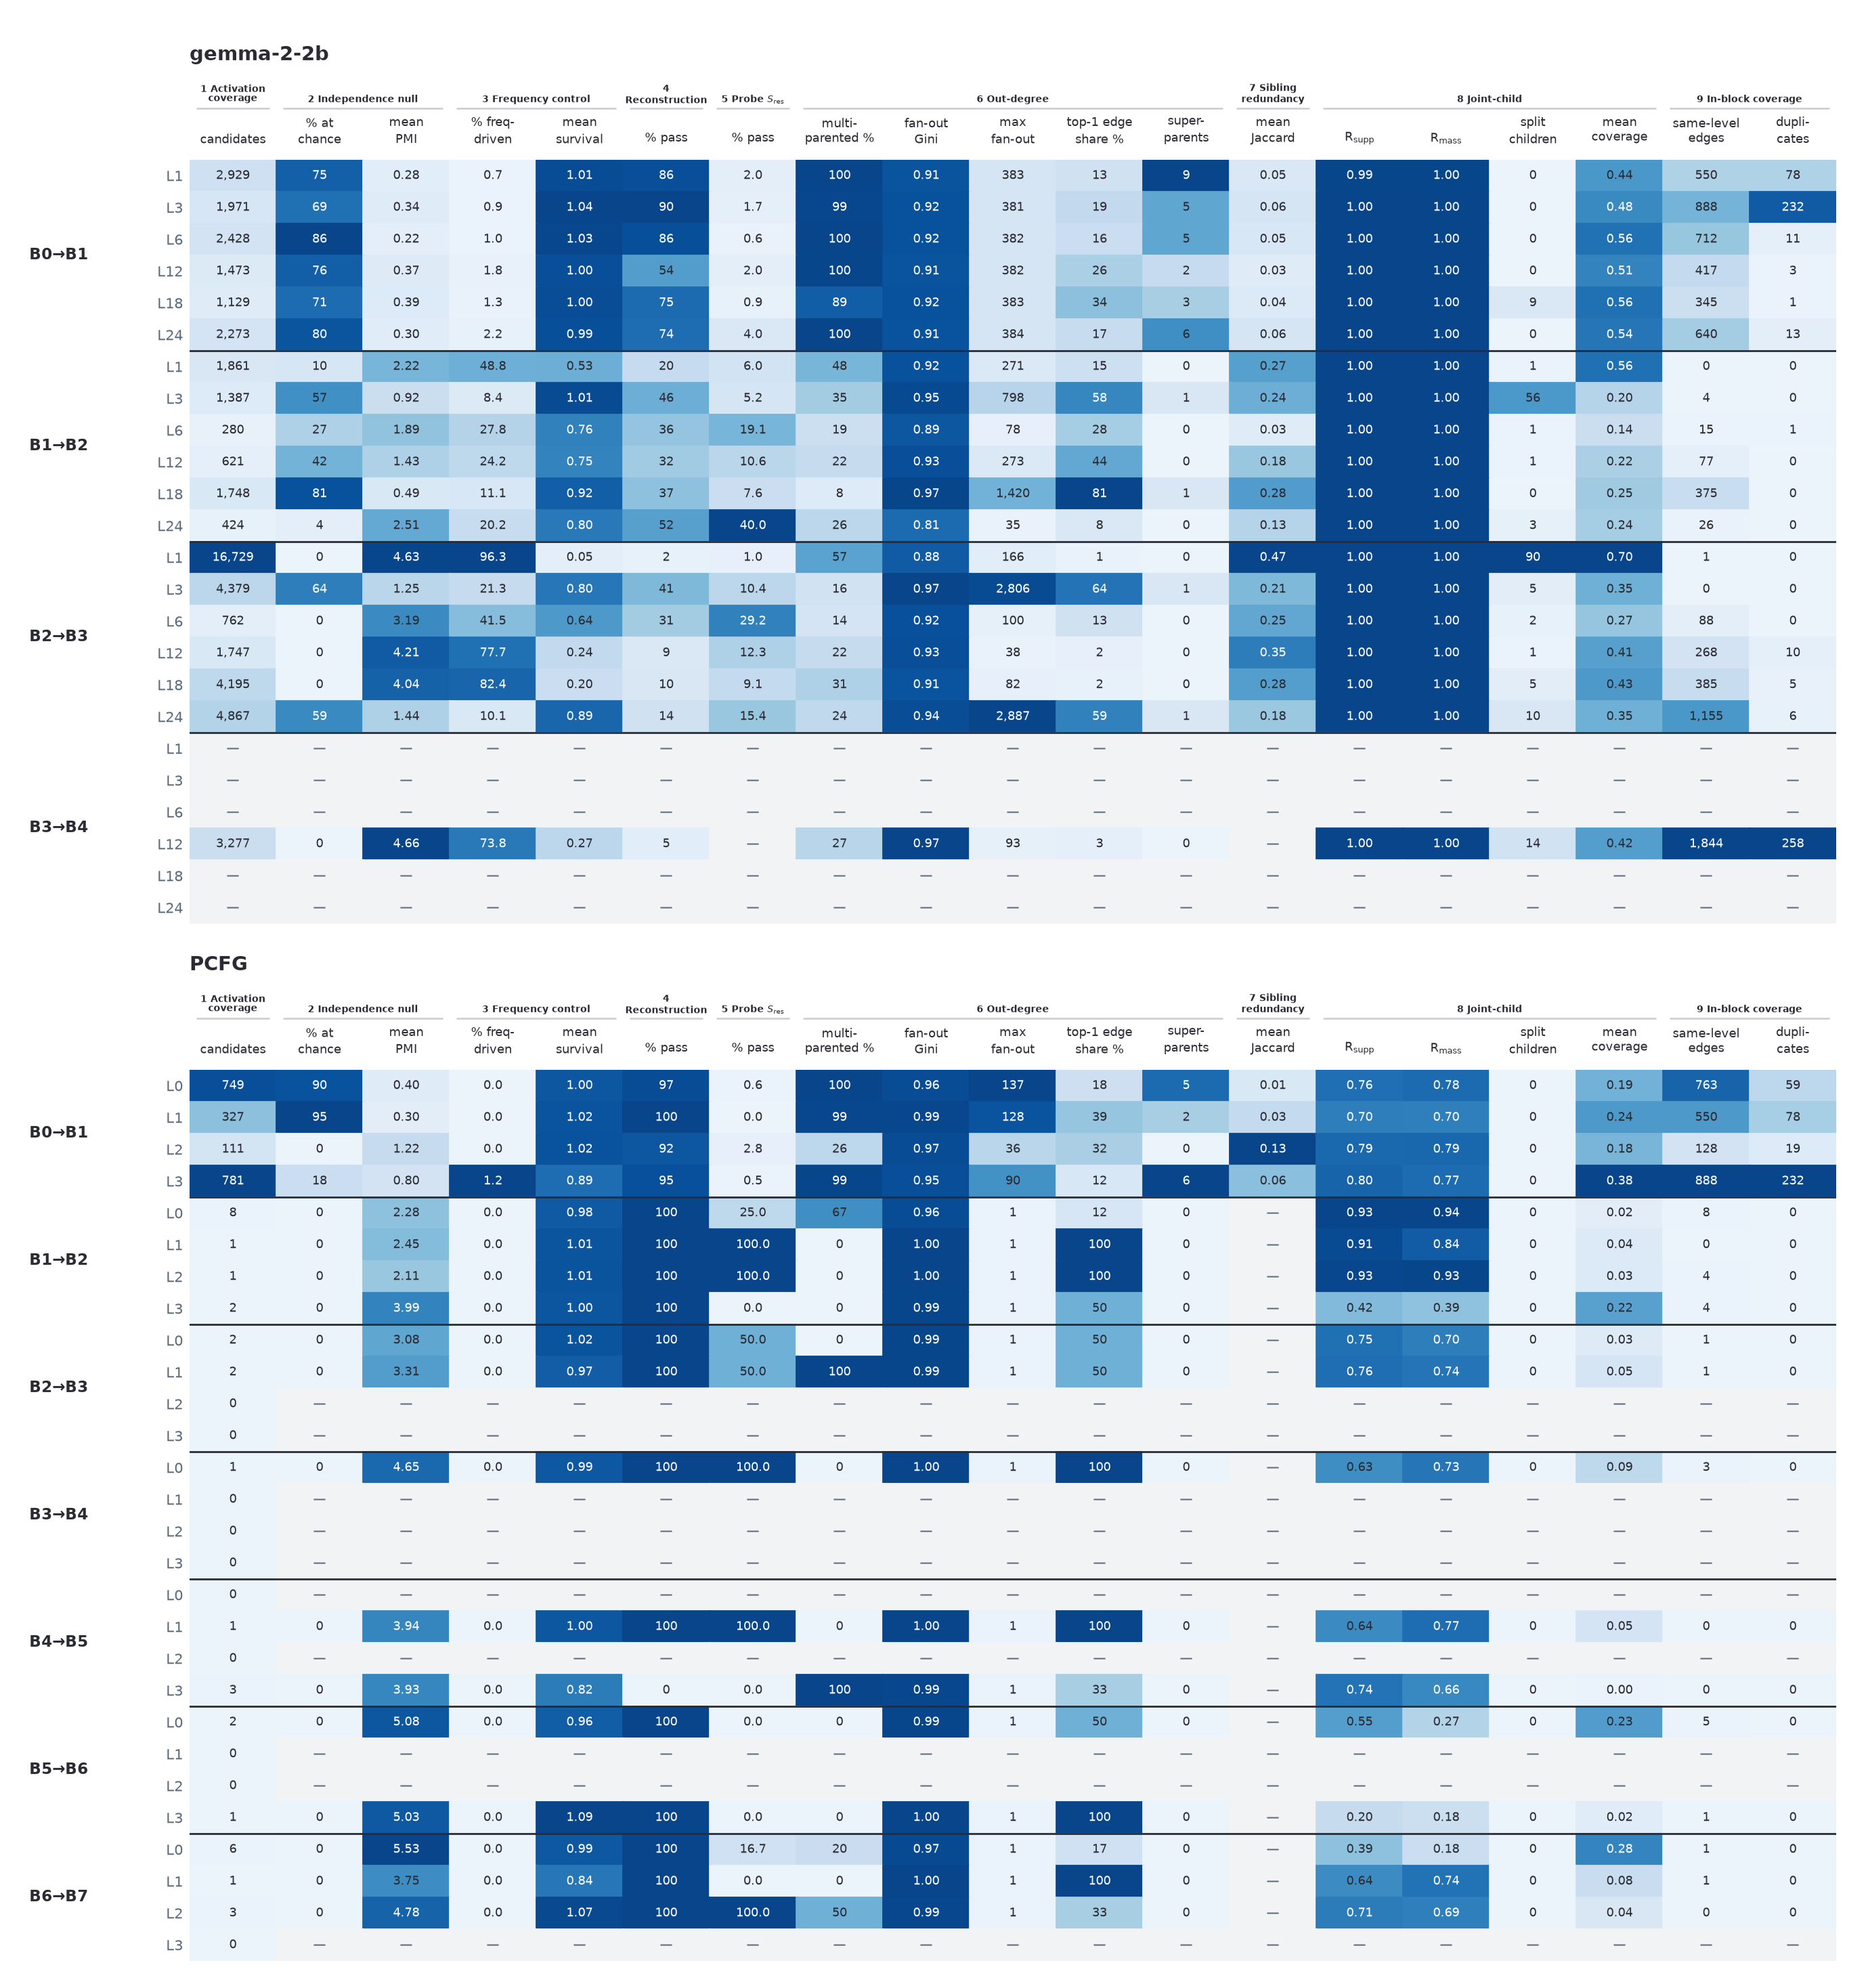
\includegraphics[width=\linewidth]{tangle_lives_in_top_block_pair}
  \caption{%
    \textbf{One instrument, untuned, on both sources.}
    Every metric per block pair \emph{and} per layer, one panel per SAE source; no cell is an
    average, so a row is one block pair read at one layer and an empty candidate set shows as
    a dash rather than as a number. Colour ranks \emph{within} a column of its own panel (the
    columns are different quantities on different scales, and the two sources have different
    dictionaries), so the reading is locational. Metric 9 is a within-block quantity while
    every row is a between-block pair, so each row reports its own parent block. Three things
    read off it. The structural pathology (multi-parenting, base-rate co-firing, superparents)
    sits in the outermost pair B0$\rightarrow$B1 and it is not an average effect:
    multi-parenting is 89--100\% at \emph{every} graded layer of gemma and 99--100\% at three
    of the four PCFG layers. The deeper pairs are not clean but differently broken, failing
    the frequency control instead (up to 96.3\% of B2$\rightarrow$B3 edges at L1) with sibling
    overlap several times higher. And fan-out Gini is the one column that localises nothing,
    sitting at 0.81--0.97 on gemma and 0.95--1.00 on PCFG in every pair at every layer, which
    makes it a property of the dictionary rather than of any boundary within it. The PCFG deep
    pairs rest on one to three candidate edges, so their quiet columns record emptiness, not
    health. gemma's fourth adjacent pair B3$\rightarrow$B4 is read at layer 12 alone: its
    co-firing matrix is 6{,}144$\times$24{,}576 and needs a 49 GB card, so it is off by
    default and was run once. The five dashes beside it mean not run, not empty. The
    distinction is drawn rather than left out, because a pair silently absent from a grid
    reads as a pair with nothing in it, which is a claim the run never tested.
  }
  \label{fig:tangle-lives-in-top-block-pair}
\end{figure}

% [MAIN 1b]
\begin{figure}[tbp]
  \centering
  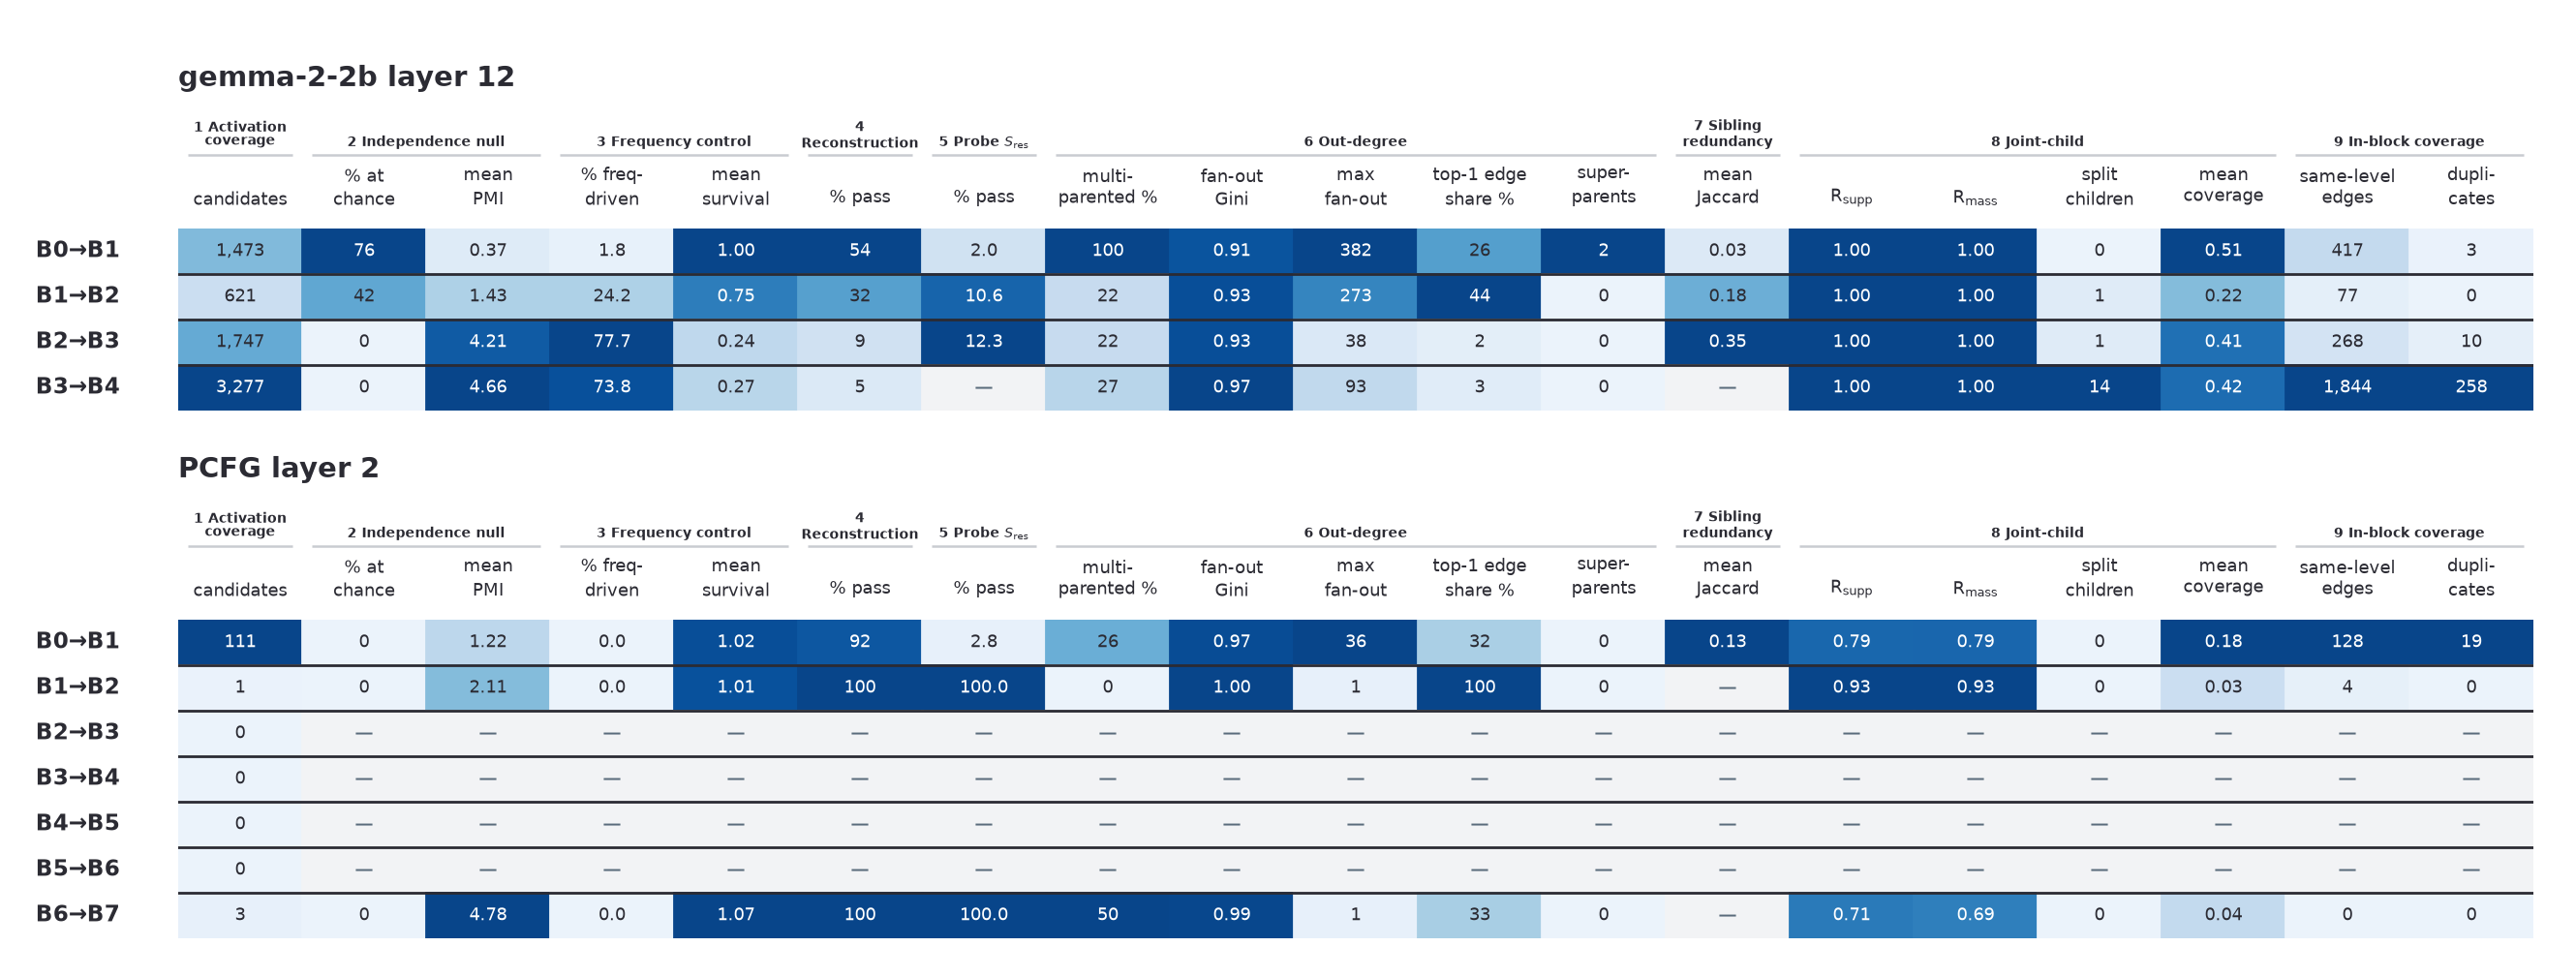
\includegraphics[width=\linewidth]{metrics_result_mid_layers}
  \caption{%
    \textbf{The metrics result at mid layers.} This figure displays the results of all metrics
    across the middle layer and all its blocks: \texttt{gemma-2-2b} at layer 12 and the PCFG
    SAE at layer 2.
  }
  \label{fig:metrics-result-mid-layers}
\end{figure}

% [MAIN 2]
\begin{figure}[tbp]
  \centering
  \includegraphics[width=\linewidth]{funnel_coverage_to_sres}
  \caption{%
    \textbf{Broad coverage does not translate into confirmed structure.} Coverage proposes
    many candidate relationships (1,129--2,929 per layer), but successive independence and
    probe tests eliminate most of them: the independence null rejects 69--86\%, and the probe
    confirms only 8--55 edges per layer ($0.6$--$4.0\%$ of those scored), leaving only a small
    subset of supported parent--child relationships. The reconstruction filter (passing
    54--90\%) is evaluated separately because it does not form a nested stage. The PCFG panel
    repeats the same collapse at small scale: 111--781 candidates per layer end in 0--4
    probe-confirmed edges.
  }
  \label{fig:funnel-coverage-to-sres}
\end{figure}

% [MAIN 3]
\begin{figure}[tbp]
  \centering
  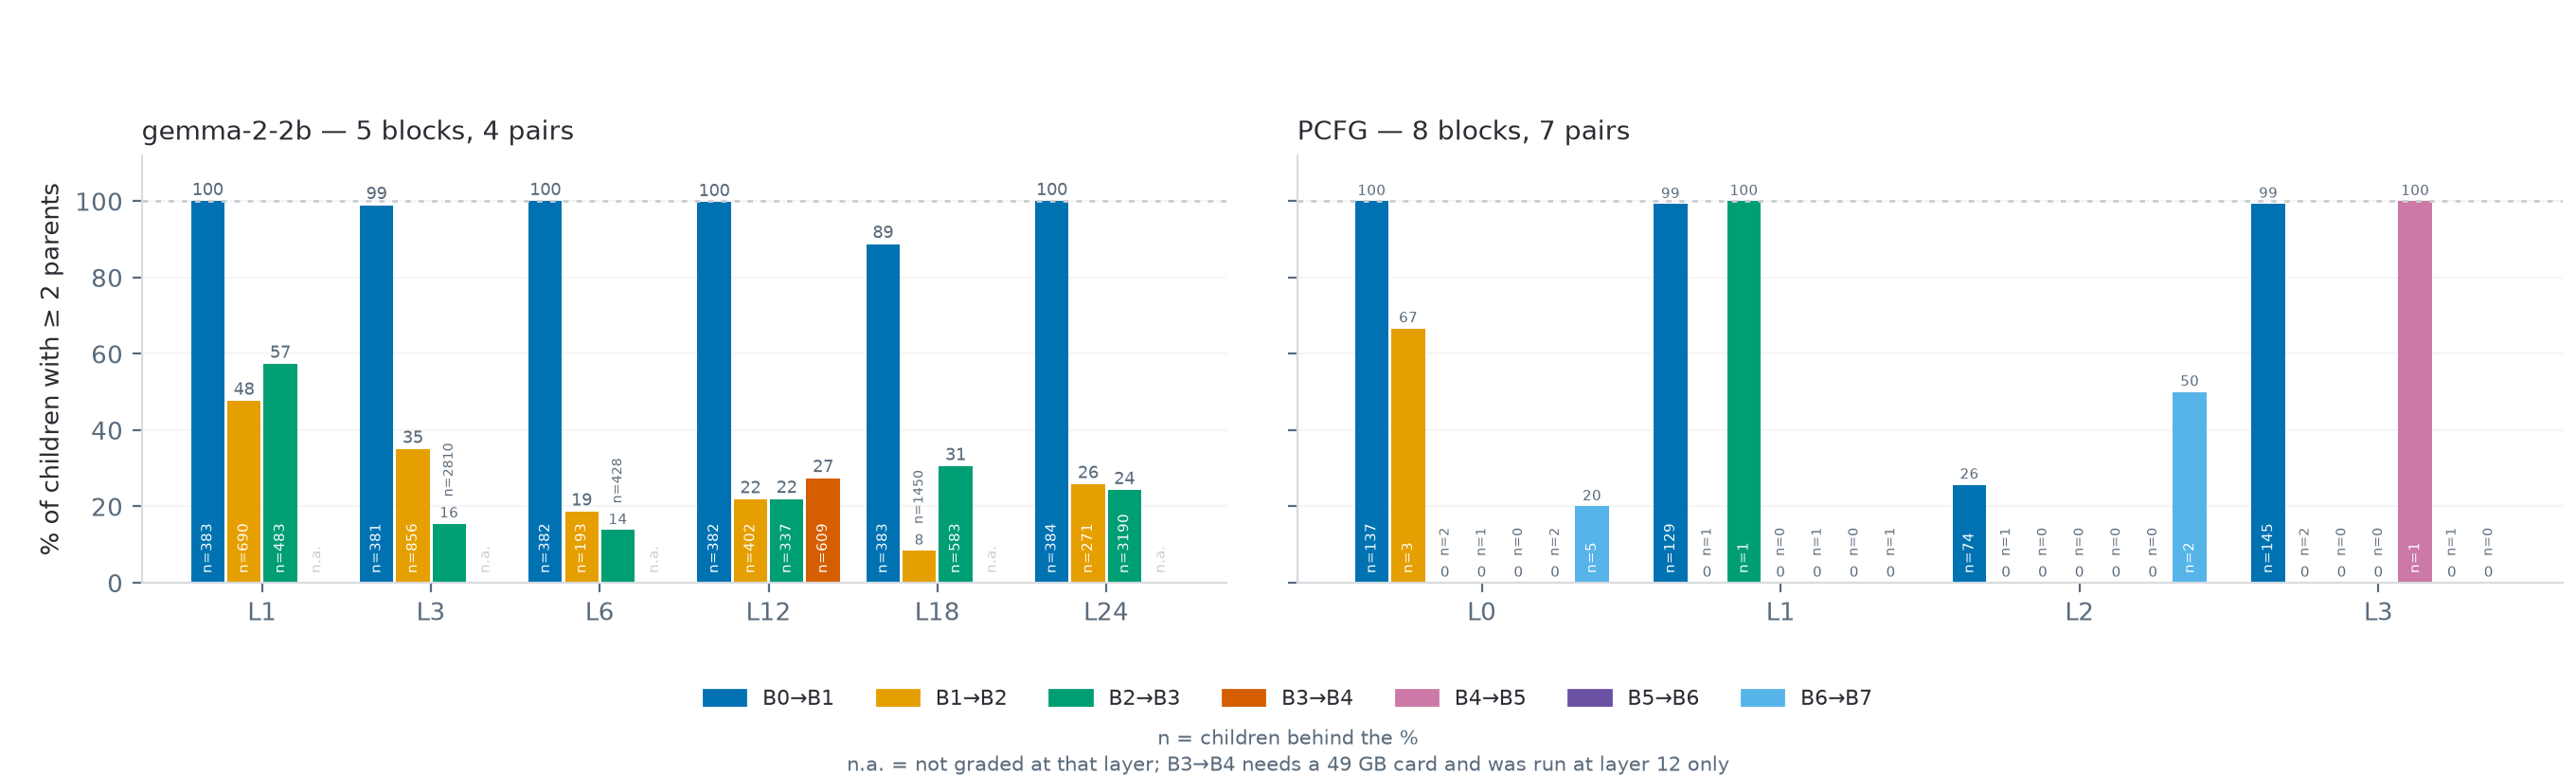
\includegraphics[width=\linewidth]{multiparenting_by_layer}
  \caption{%
    \textbf{The recovered graph is not a tree.} Child features are often associated with
    multiple parents rather than a single parent: in the top block pair B0$\rightarrow$B1,
    89--100\% of children with any parent have two or more, at every graded layer, revealing
    pervasive multi-parenting in the recovered structure. Deeper block pairs appear cleaner
    (8--57\%) on candidate sets of comparable or larger size, so the drop reflects genuinely
    looser structure rather than a smaller sample. Gemma's B3$\rightarrow$B4 pair is graded at
    layer 12 alone: its co-firing matrix is 6{,}144$\times$24{,}576, which needs a 49 GB card,
    so it is off by default and was run once. The other five layers are marked n.a. because
    they were not run, not because they cannot be. Every bar prints the number of children
    behind its percentage as $n{=}$; a 100\% computed over one child is a coin flip, not a
    result, and the label keeps it from reading as one. The PCFG panel shows the same
    signature (26--100\% in B0$\rightarrow$B1 across its layers), so the multi-parenting is a
    property of the Matryoshka nesting, not of natural language; its deeper-pair bars rest on
    a handful of children and carry their support ($n$) rather than posing as results.
  }
  \label{fig:multiparenting-by-layer}
\end{figure}

% [MAIN 4]
\begin{figure}[tbp]
  \centering
  \includegraphics[width=\linewidth]{recovered_graph_toy_vs_pcfg_vs_gemma}
  \caption{%
    \textbf{The recovered graph, drawn edge by edge.} Hierarchy is partially recovered, but
    not as a clean tree, especially at scale. \emph{Left:} the trained toy recovers 9/9 true
    edges with no false positives, while \emph{Middle:} a Matryoshka SAE trained on a PCFG
    corpus (layer~2, B0$\rightarrow$B1) repeats the tangle at small scale (107 candidate
    edges, 21 parents $\times$ 73 children, 3 probe-confirmed), and \emph{Right:} Gemma-2-2B
    (layer 12, B0$\rightarrow$B1) shows substantial multi-parenting among the 1,111 candidate
    edges that reached the probe (63 parents $\times$ 355 children), with only the 22
    probe-confirmed edges in green. Read left to right, the worlds ascend in scale and
    complexity (20 hand-built features, a 1,792-latent SAE over a small transformer, a
    32,768-latent SAE over a 2B-parameter LLM), and the recovered structure degrades in step:
    a clean tree, a small tangle, a dense one. Blue marks a candidate edge that reached the
    probe but was not confirmed, green a probe-confirmed edge, and on the toy panel a dashed
    line marks a true edge the SAE never learned. Each child is placed beneath its
    best-matching parent, so a clean hierarchy would appear as near-vertical lines, and a
    parent's dot area scales with its child count, so the hub parents that own most of the
    tangle are visible at a glance.
  }
  \label{fig:recovered-graph}
\end{figure}

% -------------------------------------------------------------------------
% Appendix: the instrument, calibrated
% -------------------------------------------------------------------------

% [APP 0a]
\begin{figure}[tbp]
  \centering
  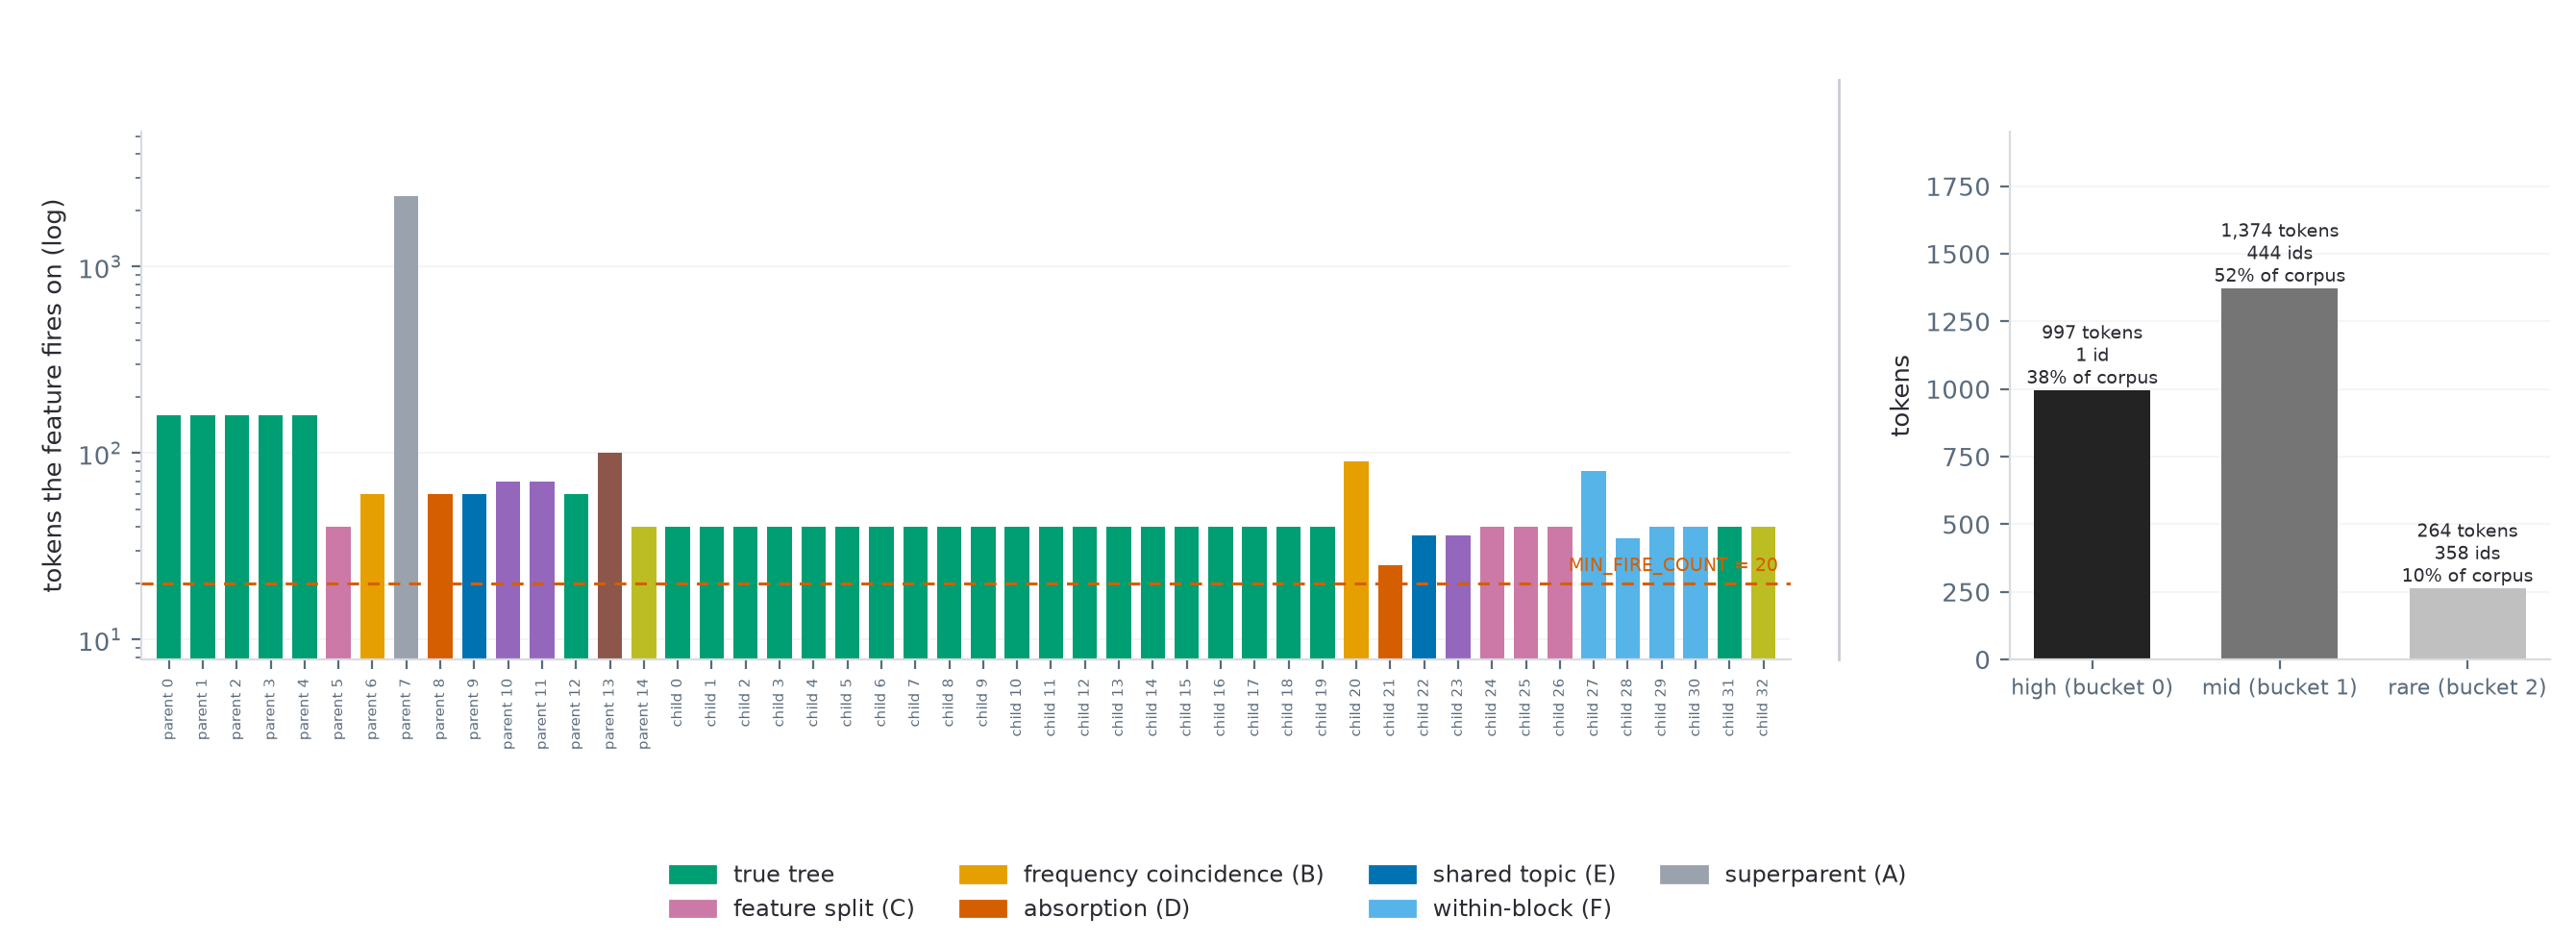
\includegraphics[width=\linewidth]{calibration_toy_corpus_firing}
  \caption{%
    \textbf{The corpus the Tier-1 calibration is run on.} Every claim in this appendix is a
    claim about a corpus, and a metric that separated two classes cleanly on a corpus with
    nothing in it has demonstrated nothing. \emph{Left:} the tokens each declared feature
    fires on, log scale, coloured by the role it was planted as; the dashed line is the
    production \texttt{MIN\_FIRE\_COUNT} $= 20$, below which no pair is scored at all. Zero of
    the 48 declared features never fire and are drawn as stubs at the floor rather than
    omitted. The super-parent is visible as the single bar an order of magnitude above
    everything else --- that is what makes it a super-parent. \emph{Right:} where the corpus's
    token mass sits across the three frequency buckets metric 5 re-weights by: 52\% of all
    tokens fall in bucket 1, carried by 444 distinct ids. That concentration is what the
    frequency control has to work against, so it is reported rather than assumed. The bucket
    bars use a single-hue sequential shade and no role colour: buckets are an order, not a
    category, and the palette in the key below applies to the left panel only.
  }
  \label{fig:calibration-toy-corpus-firing}
\end{figure}

% [APP 0b]
\begin{figure}[tbp]
  \centering
  \includegraphics[width=\linewidth]{calibration_reverse_coverage}
  \caption{%
    \textbf{What the first gate proposes, and the one true edge it cannot.} The
    reverse-coverage matrix $R = $ co-fire\,/\,child firing for every parent--child pair in
    the hand-built world, with the ground truth drawn on top of it. Coverage keeps a pair when
    $R \geq \tau = 0.5$, which proposes 63 of the 495 possible pairs. Circles are true edges
    it proposed, crosses are pairs it proposed that no true edge backs, and the square is the
    reading that matters: a true edge whose $R$ never reaches the threshold, so no later gate
    ever sees it. That is a limit of the first gate which no downstream metric can repair, and
    it is the same absorption case the scorecard files as a demonstrated blind spot rather
    than a caught pathology. The super-parent's row is the wide band of crosses --- one parent
    proposing against nearly every child, at high $R$, on co-firing alone.
  }
  \label{fig:calibration-reverse-coverage}
\end{figure}

% [APP 0c]
\begin{figure}[tbp]
  \centering
  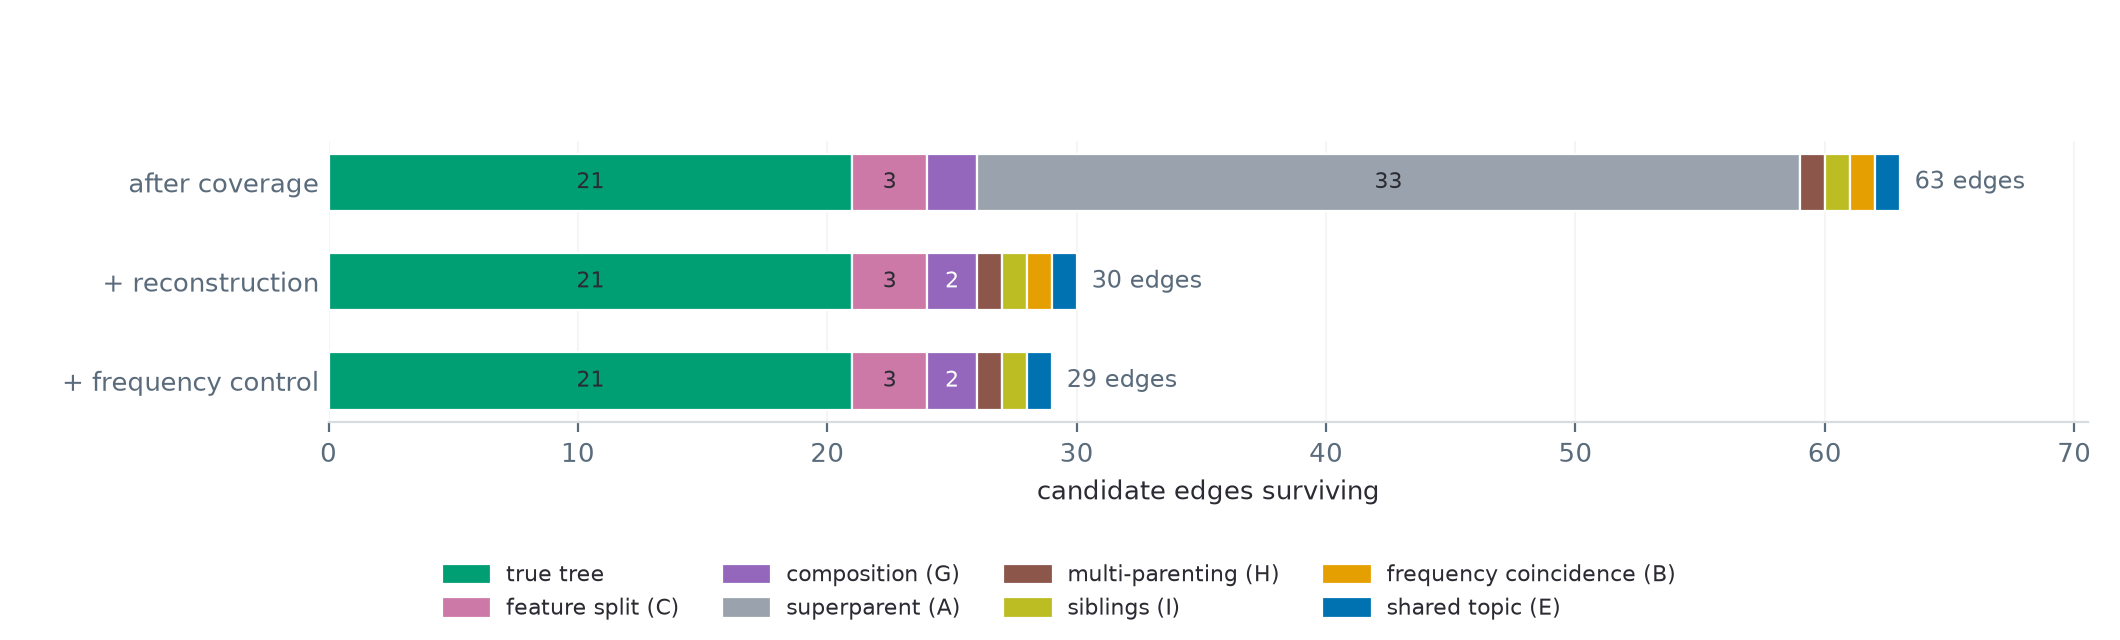
\includegraphics[width=\linewidth]{calibration_gate_funnel_by_role}
  \caption{%
    \textbf{What each gate removes, counted.} The same three composed gates the before/after
    figure draws, as counts split by the structure each candidate was planted as. Coverage
    proposes 63 candidates; the reconstruction condition takes that to 30 and the
    token-frequency control to 29. The genuine block does not move at any stage, which is the
    claim: the gates are removing planted pathology rather than thinning everything. The
    division of labour is legible in the widths --- the super-parent's candidates die entirely
    at reconstruction and not at coverage, and the frequency-coincidence pair survives both
    coverage and reconstruction and dies only at the control built for it. The two negative
    controls are the segments that never shrink; they are limitations this composition
    demonstrates, not failures of it.
  }
  \label{fig:calibration-gate-funnel-by-role}
\end{figure}

% [APP 0d]
\begin{figure}[tbp]
  \centering
  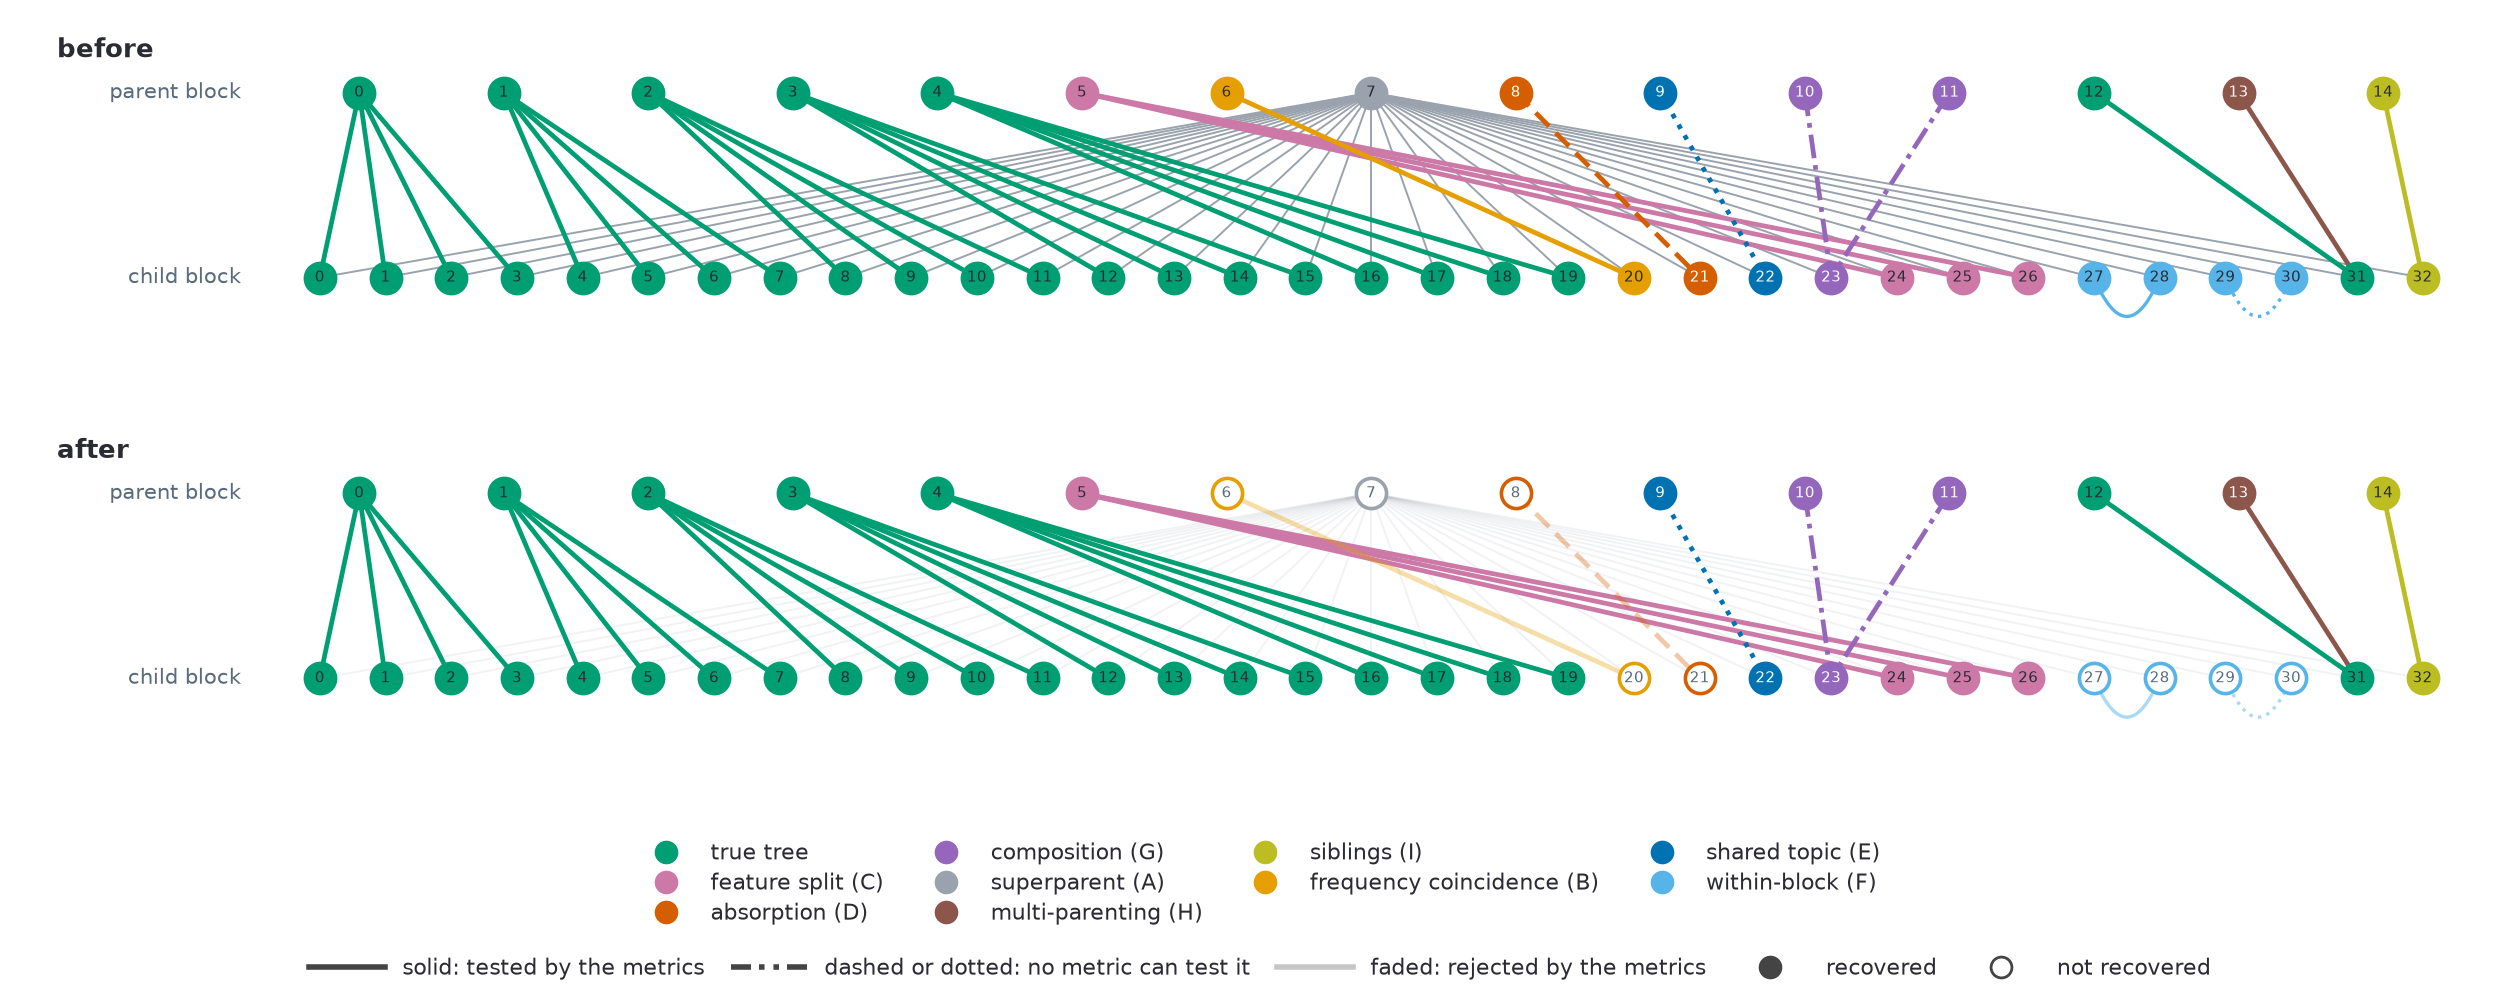
\includegraphics[width=\linewidth]{calibration_toy_world_before_after}
  \caption{%
    \textbf{Which gate caught which injected pathology.} The same hand-built world as the
    previous figure, drawn twice in one palette: one colour per injected structure, in both
    panels. \emph{Top:} the world as declared --- 25 true parent--child edges over 48
    features, plus the eight structures planted to be caught or to demonstrate that nothing
    catches them. \emph{Bottom:} the same world after the three composed gates (reverse
    coverage, the reconstruction condition, the token-frequency control), where a faded edge
    is one the gates removed and the note above each parent names the gate that removed it.
    Coverage proposes 63 candidates; 34 are rejected, and 24 of the 25 true edges survive. The
    division of labour is the reading: all 33 super-parent pairs die at the reconstruction
    condition rather than at coverage, the frequency-coincidence pair passes coverage and
    reconstruction and dies only at the frequency control, and the feature-split edges are
    recovered --- correctly, since they are real refinements --- with the split reported
    against the parent by a different metric. The dashed structures are the negative controls:
    the absorbed edge (8, 21) is never proposed at all, while the shared-topic pair (9, 22)
    and the composition edges (10, 23) and (11, 23) pass every gate. The multi-parenting
    intruder (13, 31) and the co-extensive pair (14, 32) also pass every gate and are flagged
    by reports (the child's in-degree, the energy share) rather than rejected.
  }
  \label{fig:calibration-toy-world-before-after}
\end{figure}

% [APP 0d']
\begin{figure}[tbp]
  \centering
  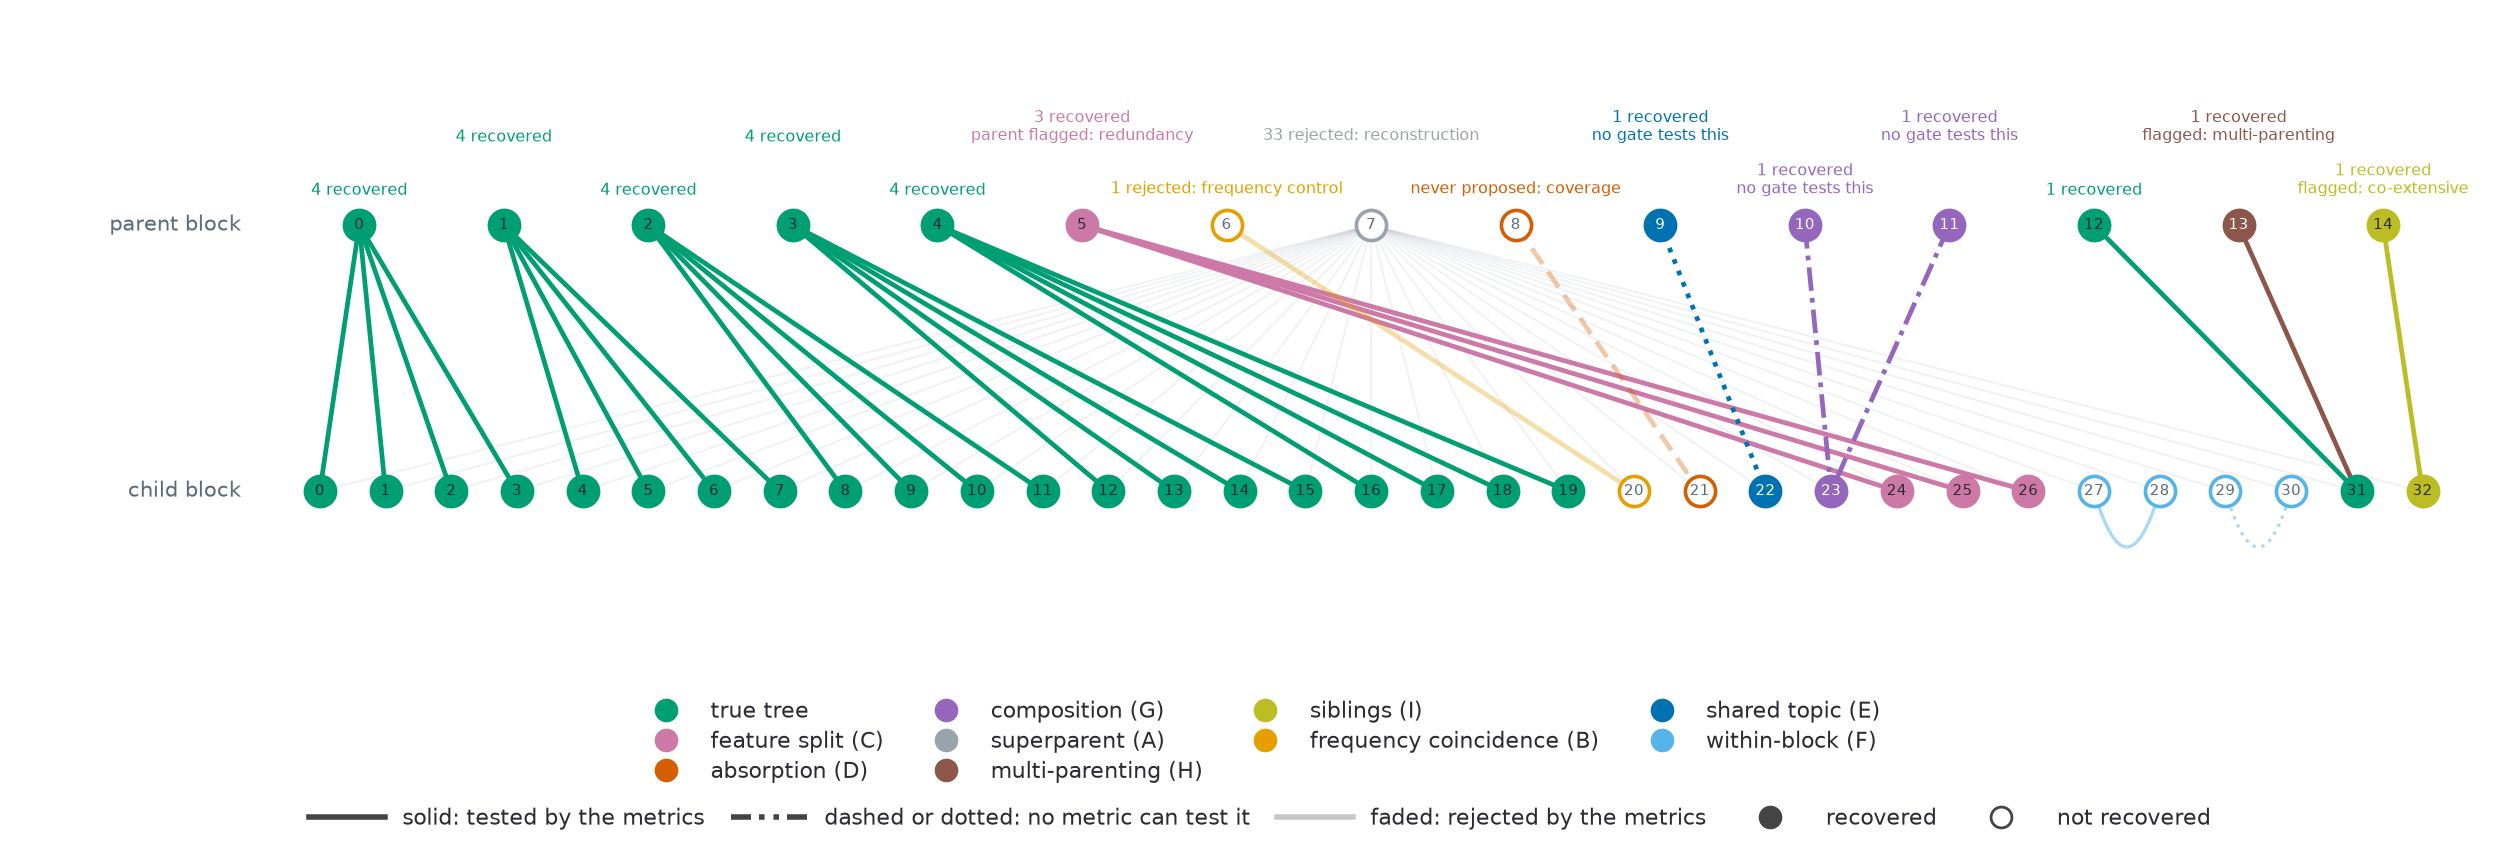
\includegraphics[width=\linewidth]{calibration_toy_world_gate_verdicts}
  \caption{%
    \textbf{What the set of metrics recovered.} The same hand-built world as the previous
    figure, drawn in one palette with one colour per injected structure: the parent block as
    the top row, the child block as the bottom row --- 25 declared true parent--child edges
    over 48 features, plus the eight structures planted to be caught or to demonstrate that
    nothing catches them. A faded edge is one the three composed gates (reverse coverage, the
    reconstruction condition, the token-frequency control) removed, so the declared world is
    every edge, bright or faded, and the note above each parent names the gate that decided
    its edges. Coverage proposes 63 candidates; 34 are rejected, and 24 of the 25 true edges
    survive. The division of labour is the reading: all 33 super-parent pairs die at the
    reconstruction condition rather than at coverage, the frequency-coincidence pair passes
    coverage and reconstruction and dies only at the frequency control, and the feature-split
    edges are recovered --- correctly, since they are real refinements --- with the split
    reported against the parent by a different metric. The dashed structures are the negative
    controls: the absorbed edge (8, 21) is never proposed at all, while the shared-topic pair
    (9, 22) and the composition edges (10, 23) and (11, 23) pass every gate. The
    multi-parenting intruder (13, 31) and the co-extensive pair (14, 32) also pass every gate
    and are flagged by reports (the child's in-degree, the energy share) rather than rejected.
  }
  \label{fig:calibration-toy-world-gate-verdicts}
\end{figure}

% [APP 0e]
\begin{figure}[tbp]
  \centering
  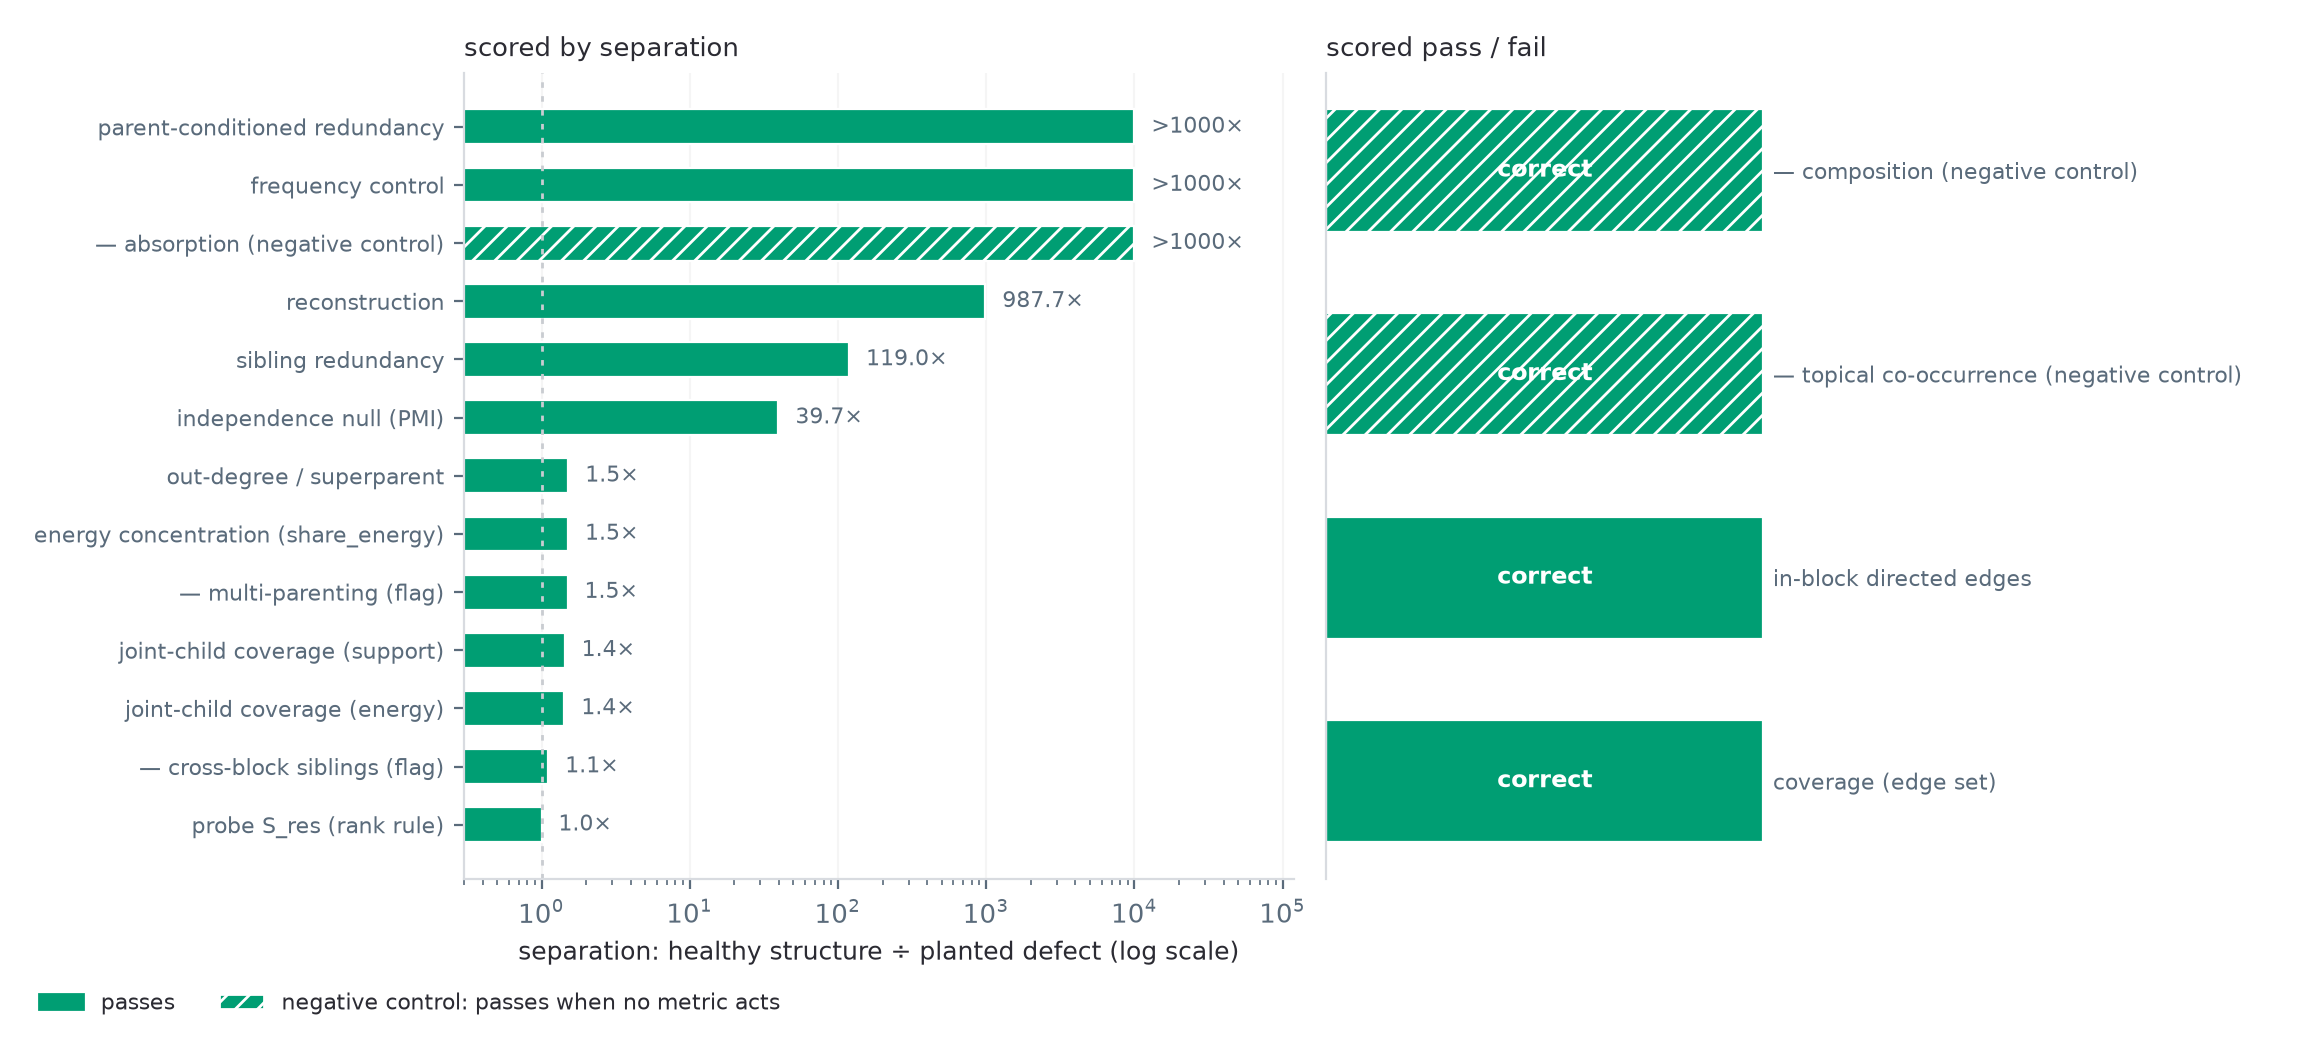
\includegraphics[width=\linewidth]{calibration_synthetic_toy_scorecard}
  \caption{%
    \textbf{Calibrating the metrics where the answer is known.} The test world is built by
    hand: activations are composed from a known concept hierarchy (six parent features, each
    with children that fire only when it fires) plus eight planted look-alike structures that
    a naive co-firing analysis would mistake for parent--child links, such as a feature pair
    that co-fires only through shared frequent tokens, a pair lifted together by a shared
    topic, and an always-on ``super-parent''. Each row is one of the metrics
    (Table~\ref{tab:battery}) applied to this world, and a row passes when the metric tells
    its planted target apart from healthy structure; 17 of 17 rows pass. \emph{Left:} metrics
    that return a score. The bar is the separation: the ratio between the metric's value on
    the pairs it must flag and its value on the pairs it must keep, so $1\times$ means the two
    are indistinguishable and the metric carries no signal. \emph{Right:} metrics whose output
    is a discrete answer (an edge set, a direction), scored simply as correct or not; the two
    panels are separate because a discrete answer has no meaningful ratio. The three hatched
    rows are negative controls, planted blind spots expected to slip through: an absorbed
    child that coverage cannot even propose (the child fires exactly where its parent is
    silent), a shared-topic pair, and a composed child's two component edges that every filter
    accepts. They pass when nothing catches them, documenting the metric set's limits, and a
    code change that made them catchable would fail them visibly. Passing this tier is what
    licenses running the same metrics on real models, where no ground truth exists.
  }
  \label{fig:calibration-synthetic-toy-scorecard}
\end{figure}

% [APP 0f]
\begin{figure}[tbp]
  \centering
  \includegraphics[width=\linewidth]{calibration_seed_sweep}
  \caption{%
    \textbf{The scorecard is not an accident of one draw.} Every row of the Tier-1 scorecard,
    re-run on independently drawn worlds --- a new corpus, new decoder directions and a new
    residual draw per seed, with the production thresholds unchanged. The cell carries the
    verdict and the shade carries the margin: how decisively that metric separated the two
    classes it was graded on, on a $\log_{10}$ scale, because the margins span orders of
    magnitude and a grid of identical verdicts would hide exactly that. A row that passes at a
    margin of $1.05$ and one that passes at $10^{3}$ are not the same evidence. The scale is
    capped at $10^{3}\times$, the same ceiling the scorecard itself prints as \texttt{>1000x}:
    three rows score $10^{9}$, which is not a measured magnitude but the guard in the
    denominator when the rejected class scores zero, and letting it set the top of the ramp
    pushed every honestly-measured margin into the palest two shades. Rows scored
    categorically have no magnitude to report and are left grey rather than given an invented
    one. Everything else in this appendix is reported at seed 0; this is the figure that says
    what that number is worth.
  }
  \label{fig:calibration-seed-sweep}
\end{figure}

% [APP 0g]
\begin{figure}[tbp]
  \centering
  \includegraphics[width=\linewidth]{calibration_trained_toy_recovery}
  \caption{%
    \textbf{The same world, after a real training run.} The toy world's ground truth is a
    tree: a set of parent$\rightarrow$child links between features (its edges). Here a
    Matryoshka SAE is actually trained on the world's activations, each learned latent is
    matched to the true feature it represents, and an edge counts as recovered when the SAE
    learned latents for both of its features and the metrics keep the link between them.
    Precision 1.00, recall 1.00: 9 of 9 true edges recovered with 0 false positives. The SAE
    recovered 20 of 20 true features, so no edge was out of reach and recall is not bounded by
    the SAE here. \emph{Right:} the lateral control, asking whether the Matryoshka nesting
    itself places a parent in an earlier block than its children. Beyond edge recovery, the
    parent-conditioned sibling metric stays at or below 0.00 for every true parent, against a
    threshold of 0.50: on this checkpoint the SAE kept each parent's mutually exclusive
    children apart rather than conflating them.
  }
  \label{fig:calibration-trained-toy-recovery}
\end{figure}

% [APP 0h]
\begin{figure}[tbp]
  \centering
  \includegraphics[width=\linewidth]{calibration_toy_tree_recovered}
  \caption{%
    \textbf{What an edge is, and what the metrics did with it.} The toy world is a generative
    process: each node is a feature that fires with the probability printed beneath it,
    \emph{conditional on its parent firing}. Feature~1 at $p=0.2$ under a parent at $p=0.15$
    therefore fires on $3\%$ of draws, not $20\%$. An \textbf{edge} is containment: a child
    fires only on draws where its parent fires, so $P(\text{parent}\mid\text{child})=1$ while
    $P(\text{child}\mid\text{parent})$ stays small, and it is that asymmetry the metrics
    measure. Hollow nodes (the root, and one hidden sibling per family) carry no feature
    index, which is why the 23 links drawn on the left reduce to 9 scoreable edges.
    \textbf{Left}: the known tree. \textbf{Right}: the same tree after a Matryoshka SAE
    (\texttt{relu}) is trained on the world's activations, each latent is matched to the true
    feature its decoder points at, and the metrics are run on the learned latents alone. It
    returned 9 of 9 true edges with 0 false positives. The reading that matters is the
    decomposition: the SAE learned 20 of 20 features, leaving 9 edges with both endpoints
    present, and the metrics returned \emph{all} 9 of them. Nothing was dropped and nothing
    was invented: on this checkpoint the metrics reproduce the tree exactly. One run is not a
    guarantee. An independent checkpoint on a different architecture (\texttt{batch\_topk},
    $k=2$, this repo's trainer) learned 17 of 20 features and returned 6 of 9 edges with 0
    false positives: it too returned every edge whose endpoints both existed (6 of 6).
  }
  \label{fig:calibration-toy-tree-recovered}
\end{figure}

% -------------------------------------------------------------------------
% Appendix: what the metrics find
% -------------------------------------------------------------------------

% [APP 1b]
\begin{figure}[tbp]
  \centering
  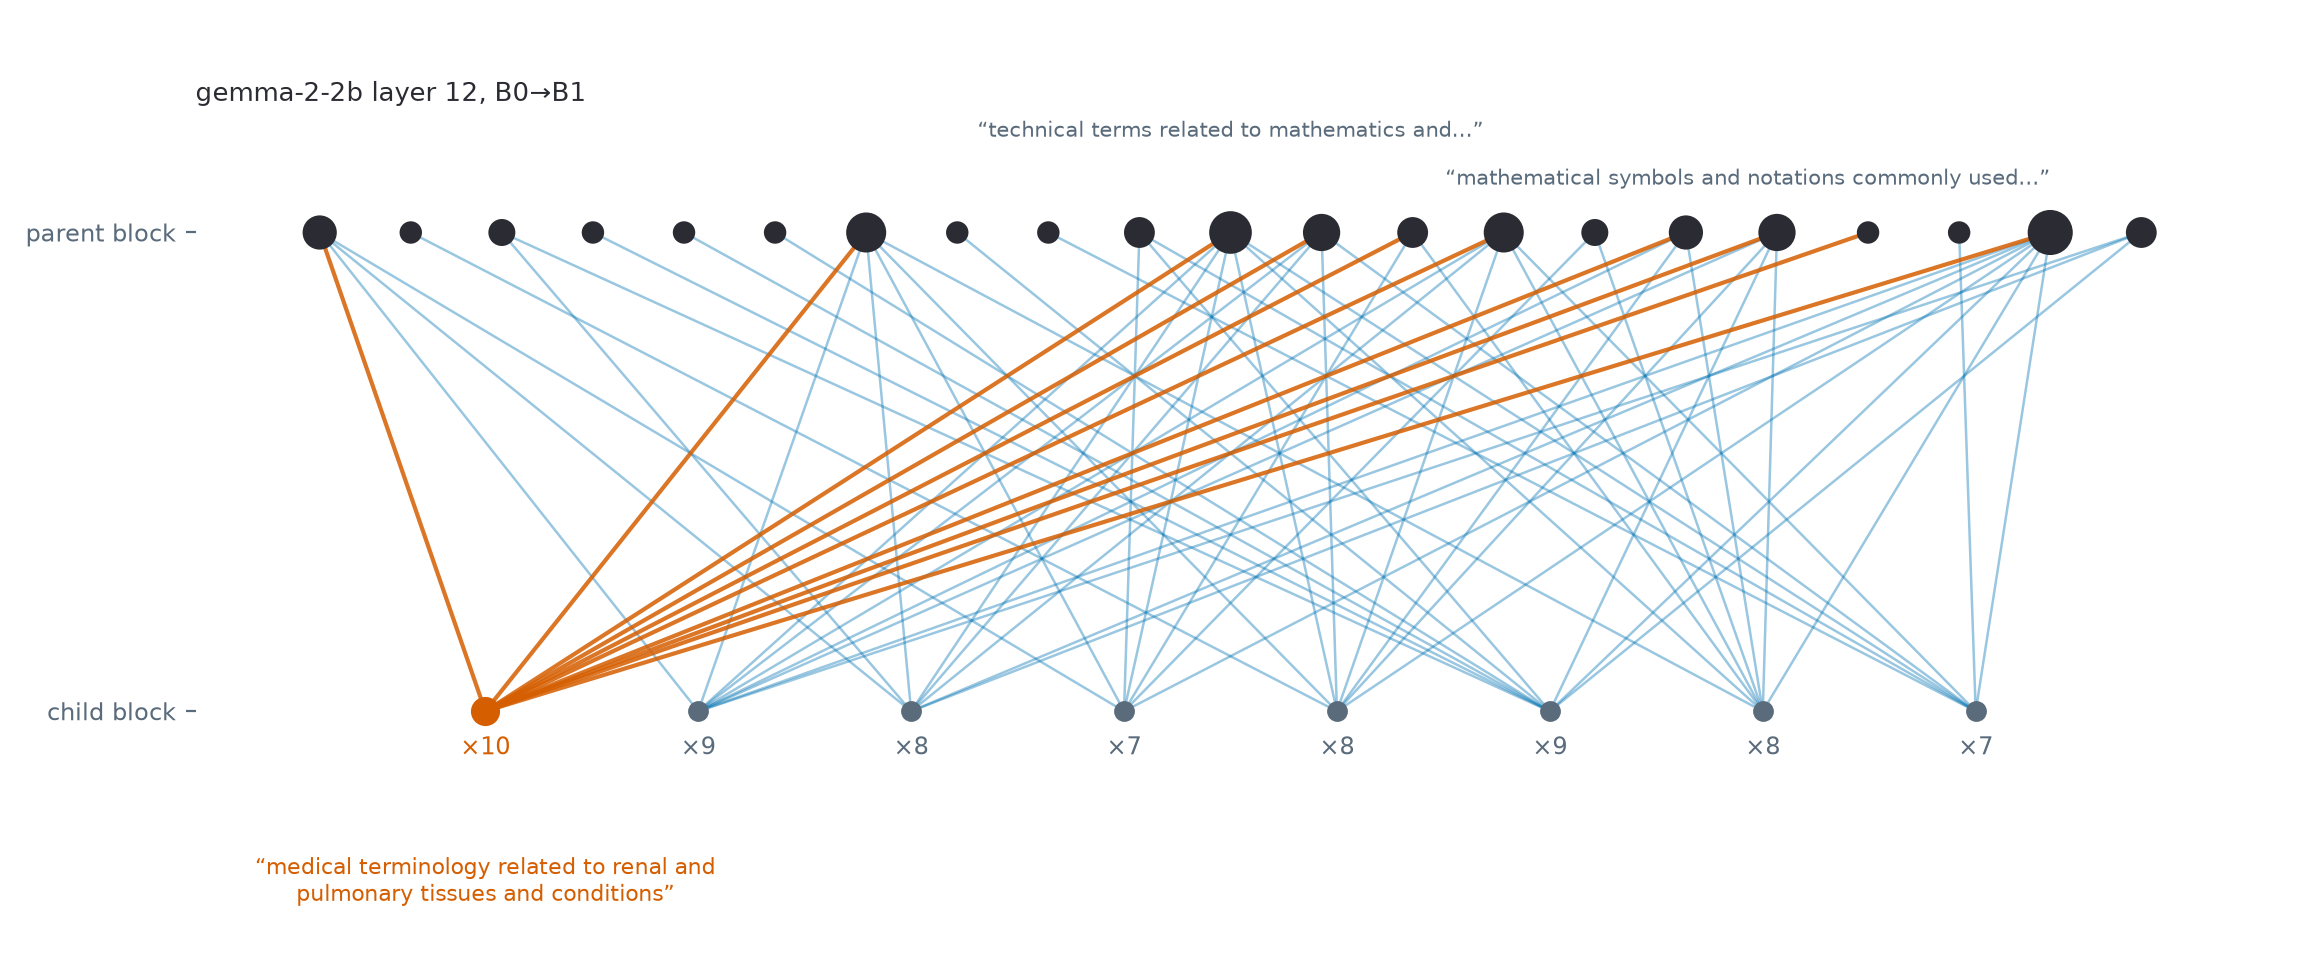
\includegraphics[width=\linewidth]{a_slice_of_the_tangle}
  \caption{%
    \textbf{A slice of the tangle.} A parent with many children is what a hierarchy looks
    like; a child with many parents is what breaks one. A tree grants each child exactly one
    parent, and in this slice of gemma-2-2b (layer 12, B0$\rightarrow$B1), selected by a
    stated rule (the eight most-claimed children and every parent claiming them), the featured
    child alone is claimed by 10 parents at once, its neighbours by 7--9 each, and the
    \emph{median} child of the whole pair has 3. This is the per-child view of the 81\%
    multi-parenting rate: the violation is not a tail event but the typical case.
    Neuronpedia's labels name the absurdity: a child read as ``medical terminology related to
    renal and pulmonary tissues…'' is claimed by parents read as ``terms related to data
    management and database…'', ``technical terminology related to programming…'', ``technical
    terms related to mathematics and…'', among others; the labels are automatic and noisy, but
    the point is structural, not semantic.
  }
  \label{fig:a-slice-of-the-tangle}
\end{figure}

% [APP 1b']
\begin{figure}[tbp]
  \centering
  \includegraphics[width=\linewidth]{one_child_many_parents}
  \caption{%
    \textbf{A child with 10 parents.} The single-child view of the slice in
    Fig.~\ref{fig:a-slice-of-the-tangle}, with every claiming parent's label spelled out. A
    tree grants each child exactly one parent; the most-claimed child feature of gemma-2-2b
    (layer 12, B0$\rightarrow$B1) is claimed by 10 at once, while the \emph{median} child with
    any parent has 3. Neuronpedia's labels name the absurdity: a child read as ``medical
    terminology related to renal and pulmonary tissues…'' is claimed by parents read as
    ``terms related to data management and database…'', ``technical terminology related to
    programming…'', ``technical terms related to mathematics and…'', among others; the labels
    are automatic and noisy, but the point is structural, not semantic.
  }
  \label{fig:one-child-many-parents}
\end{figure}

% [APP 1c]
\begin{figure}[tbp]
  \centering
  \includegraphics[width=\linewidth]{one_parent_owns_the_block}
  \caption{%
    \textbf{One parent owns the block.} The hub structure behind the tangle, isolated on
    gemma-2-2b (layer 12, B0$\rightarrow$B1). \emph{Left:} the single biggest parent feature
    claims 220 of the 355 children that have any parent (62\%). \emph{Right:} ownership of all
    1,111 candidate edges is concentrated: the top parent alone carries 20\%, the top five
    60\%, and the top ten 78\% of every proposed parent$\rightarrow$child relationship. A
    hierarchy distributes parenthood; a hub monopolises it, which is what the fan-out Gini and
    superparent metrics quantify in aggregate.
  }
  \label{fig:one-parent-owns-the-block}
\end{figure}

% -------------------------------------------------------------------------
% The bottleneck-hijacking hypothesis, tested
% -------------------------------------------------------------------------

% [APP 2]
\begin{figure}[tbp]
  \centering
  \includegraphics[width=\linewidth]{base_rate_vs_frequency_capture}
  \caption{%
    \textbf{The over-connection is a base-rate effect, not token-frequency capture.}
    Two per-edge diagnostics on the same candidate sets, B0$\rightarrow$B1. The independence
    null asks whether co-firing exceeds what the parent's own firing rate already forces, and
    rejects 69--86\% of edges. The token-frequency control asks whether the edge survives once
    globally frequent tokens are removed, and rejects 0.7--2.2\%. They disagree by
    37--104$\times$ at every layer. This tests the observation the bottleneck-hijacking
    hypothesis is built on (that the over-connected parents mostly track high-frequency tokens
    such as spaces, punctuation and \emph{the}) and does not support it: the frequency control
    exonerates 98--99\% of edges while the base-rate null rejects most of them.
  }
  \label{fig:base-rate-vs-frequency-capture}
\end{figure}

% [APP 3]
\begin{figure}[tbp]
  \centering
  \includegraphics[width=\linewidth]{superparent_fanout_vs_firing}
  \caption{%
    \textbf{Why a parent that fires often enough clears the coverage bar for nothing.}
    An edge is kept when $P(\mathrm{parent} \mid \mathrm{child}) \geq \tau = 0.5$. Under
    independence that probability is simply the parent's firing rate $\rho$, so the enrichment
    a parent needs over chance is $\tau/\rho$, the grey curve. All 34 parents flagged as
    superparents, across six layers and every block pair, lie on it. 26 of them fire on at
    least 50\% of tokens and therefore clear the bar at $\leq 1\times$ enrichment: on base
    rate alone, with no association whatsoever between parent and child. A parent firing on
    1\% of tokens would need 50$\times$ enrichment for the same edge. This is the mechanism
    behind the previous figure.
  }
  \label{fig:superparent-fanout-vs-firing}
\end{figure}

% -------------------------------------------------------------------------
% What this says about metric batteries
% -------------------------------------------------------------------------

% [APP 4]
\begin{figure}[tbp]
  \centering
  \includegraphics[width=\linewidth]{shared_input_moved_every_metric}
  \caption{%
    \textbf{Six metrics designed as independent detectors failed together.}
    Change in each metric, averaged over the six layers, when a single contaminating token
    position is excluded from the corpus. The beginning-of-sequence token is an attention sink
    on which effectively every feature fires; with 400 documents it handed every pair in the
    dictionary 400 joint firings against a support guard set at 30, so the guard admitted
    pairs that never co-occur anywhere else. Five of these six quantities are computed from
    that one co-firing matrix, and all five moved. The sixth, multi-parenting, is a ratio over
    children that already have a parent, does not read the matrix, and did not move. Agreement
    among detectors that share an input is far weaker evidence than their number implies. The
    grey value in each pair is the withdrawn one, plotted to size the error and not as a
    result.
  }
  \label{fig:shared-input-moved-every-metric}
\end{figure}

% [APP 5]
\begin{figure}[tbp]
  \centering
  \includegraphics[width=\linewidth]{sres_null_rate_vs_dictionary_size}
  \caption{%
    \textbf{A top-$k$ rank rule is only as strict as the dictionary is large.}
    The $S_\mathrm{res}$ test passes an edge when both decoders fall within the top $k = 5$ of
    the probe's correlations over the whole dictionary. It is a geometry test, so an unrelated
    parent passes whenever chance places it there: the null rate is $k/D$, the grey line,
    which is $11.9\%$ on the 42-feature synthetic toy, $0.28\%$ on a 1{,}792-latent PCFG SAE
    and $0.015\%$ on gemma's 32{,}768. Each measured pass rate is drawn with a vertical drop
    to its own null, and that distance (not the rate) is what the measurement is worth. The
    rate is over every block pair a run probed, not its outermost pair alone
    (Table~\ref{tab:null}), because the null is a property of the dictionary and every pair is
    scored against the same one. The spread within a single dictionary is itself wide --- four
    runs on a 1,792-latent dictionary span 0.51--4.59\%, all 2--16$\times$ their null; six
    runs on a 32,768-latent dictionary span 1.56--14.41\%, all 103--944$\times$ their null ---
    which is why a raw pass rate compares nothing across sources, and little within one. A
    measured zero would have no position on a logarithmic axis and is drawn at a marked floor
    rather than silently dropped; no run needs that here.
  }
  \label{fig:sres-null-rate-vs-dictionary-size}
\end{figure}

% [APP 6]
\begin{figure}[tbp]
  \centering
  \includegraphics[width=\linewidth]{in_block_relations}
  \caption{%
    \textbf{Same-level structure lives in the outermost block.}
    Directed edges and co-extensive duplicates \emph{within} each block, where no block
    ordering fixes the direction and it must be derived from coverage asymmetry, across all 10
    graded runs. Reported as a rate per available pair rather than as a count: gemma's blocks
    are nested prefixes of 128 to 6{,}144 features, so the number of available pairs differs
    by a factor of 2{,}300 and raw counts invert the reading: the deepest block holds the most
    duplicate pairs and the fewest per pair. The concentration in B0 also holds on a PCFG SAE
    whose eight blocks are all 224 features, so it is not an artefact of B0 being small. What
    distinguishes B0 is being the outermost Matryoshka prefix: the one block trained to
    reconstruct on its own.
  }
  \label{fig:in-block-relations}
\end{figure}

% [APP 7]
\begin{figure}[tbp]
  \centering
  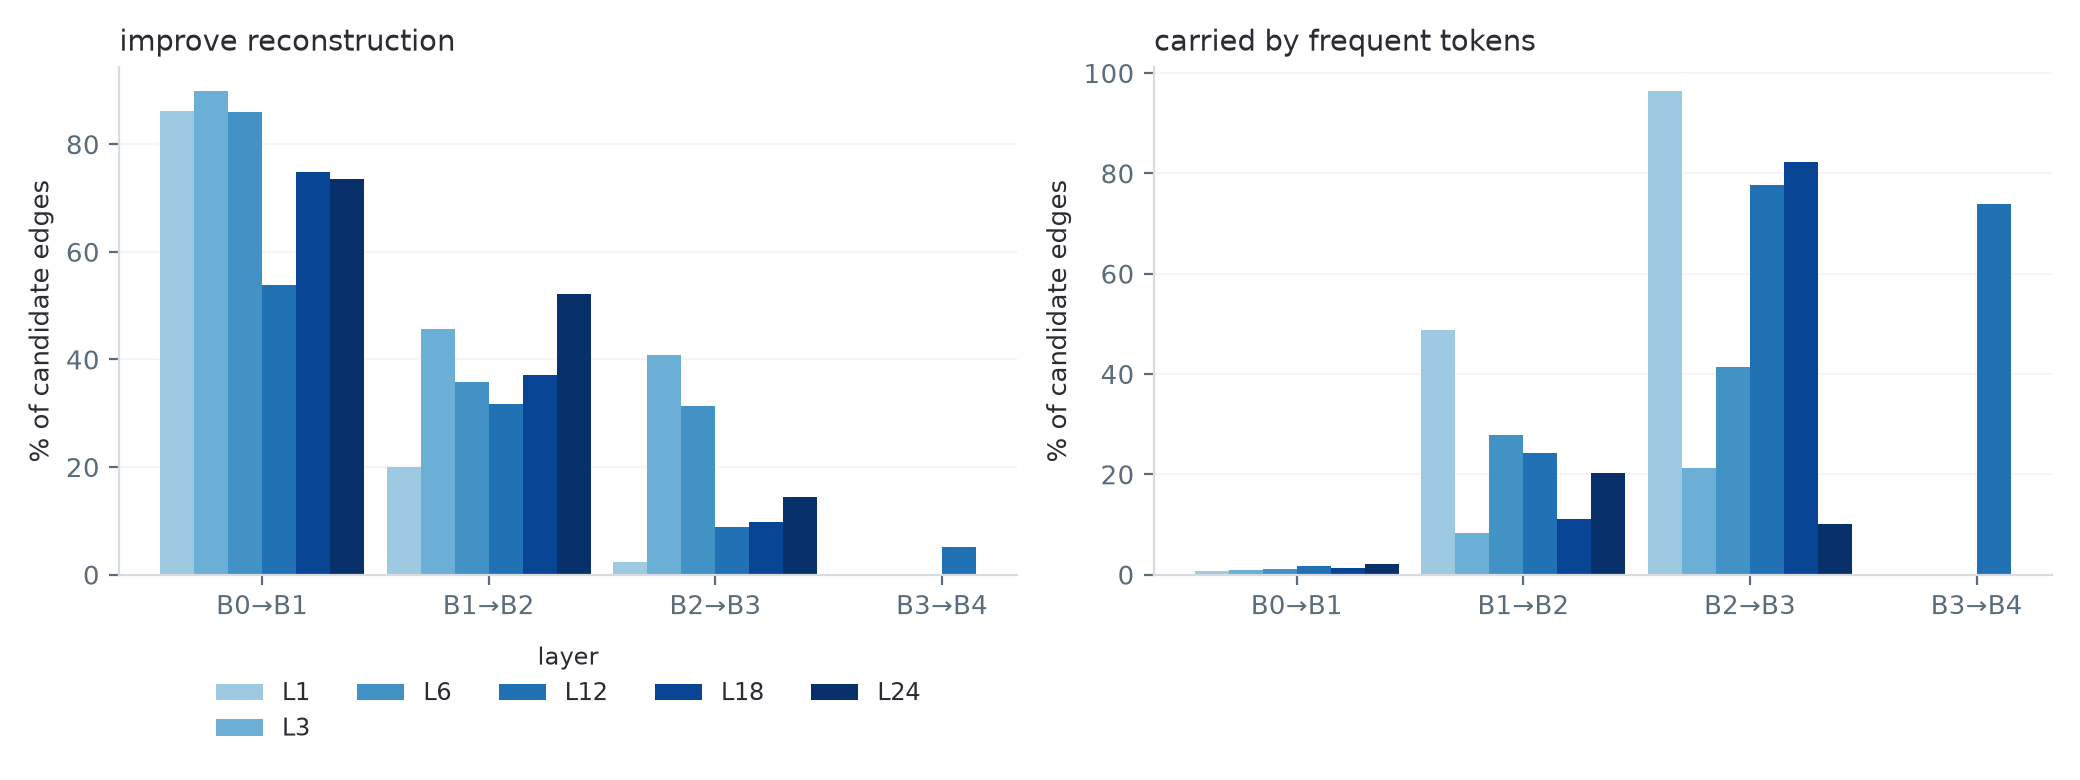
\includegraphics[width=\linewidth]{edge_survival_by_block_pair}
  \caption{%
    \textbf{What each filter removes, by block pair and by depth.}
    \emph{Left:} the share of candidate edges whose reconstruction improves when the parent is
    ablated. \emph{Right:} the share the token-frequency control judges to be carried by
    globally frequent tokens. Panels are on separate scales; layers are ordered, so depth is
    encoded as a single-hue ramp rather than as five categorical colours. The frequency
    control is nearly silent in the top block pair and rises sharply in the deeper ones.
  }
  \label{fig:edge-survival-by-block-pair}
\end{figure}

% [APP 8]
\begin{figure}[tbp]
  \centering
  \includegraphics[width=\linewidth]{cross_source_funnel_shares}
  \caption{%
    \textbf{One unchanged metric set across SAE sources.}
    The same metric code and the same global thresholds, applied to the released Matryoshka
    SAE on \texttt{gemma-2-2b} and to Matryoshka SAEs trained on a PCFG corpus. Reported as
    shares of each run's own candidate set, because the dictionaries differ in size and in
    block count and counts would not compare. Thresholds are deliberately not tuned per
    source: holding them fixed is what makes any cross-source comparison mean something. The
    reconstruction filter should be read with care on PCFG, where the weakest candidate edge
    sits $3.5\times$ above the threshold, so the filter is inert there and the surviving edges
    have passed coverage alone.
  }
  \label{fig:cross-source-funnel-shares}
\end{figure}

% [APP 9]
\begin{figure}[tbp]
  \centering
  \includegraphics[width=\linewidth]{cross_source_layer_response}
  \caption{%
    \textbf{The shape of the B0$\rightarrow$B1 relation is the same on both base models; its strength is not.}
    Six measurements of block pair B0$\rightarrow$B1, on the released Matryoshka SAE over
    \texttt{google/gemma-2-2b} and on Matryoshka SAEs trained over a 4-block transformer
    fitted to a PCFG corpus. Both sources have an SAE at layers 1 and 3, so the grey
    connectors are drawn between runs at the same block index and need no matching argument;
    their length is the disagreement. Every panel is a share and every panel is on the same
    axis anchored at zero, so lengths compare across panels. edges carried by frequent tokens,
    children with $\geq$ 2 parents, sibling redundancy (mean Jaccard) agree to within 1.0
    points, while edges at chance for the base rate differs by 35 and edges improving
    reconstruction by 10. \textbf{That agreement is worth less than it looks}: all 3 of the
    close measures sit against a floor or a ceiling on both sources, so scaled by the range
    each one varies over across every graded run (Table~\ref{tab:align}) only children with
    $\geq$ 2 parents stands out, and the reconstruction filter moves from nearly the worst to
    among the best. The reading we would take, carrying that caveat, is that the many-to-many
    fan-out B0$\rightarrow$B1 is a property of the Matryoshka nesting rather than of
    \texttt{gemma-2-2b}: what the base model changes is how much of it there is (6.0\% against
    1.5\% of all B0$\times$B1 feature pairs become candidate edges), not its character.
    \textbf{Both PCFG runs are a single grammar configuration} (zipf exponent 1.5, delimiters:
    eos), one point of the three-axis sweep Exp 2 specifies (terminal distribution, formatting
    density, grammar depth), so this compares gemma against one PCFG corpus and not against
    PCFG. In particular the formatting axis, which the project now treats as the mechanism
    behind bottleneck hijacking, is at its second-lowest rung here. \textbf{Two shared layers
    cannot establish a trend}, and the deeperblock pairs are excluded because the PCFG runs
    hold 0--3 candidate edges in each of them. The token budgets also differ by 21$\times$,
    which cuts against the density gap rather than explaining it: the joint-support guard is
    an absolute count, so more tokens make it easier to clear, and the source with more tokens
    is the sparser one.
  }
  \label{fig:cross-source-layer-response}
\end{figure}

% [APP 10]
\begin{figure}[tbp]
  \centering
  \includegraphics[width=\linewidth]{cross_source_alignment_check}
  \caption{%
    \textbf{Which alignment the comparison rests on, measured rather than assumed.}
    Comparing two base models of different depth requires an alignment, and the two defensible
    ones disagree here about which runs to pair: by block index the PCFG layers pair with
    gemma's L1 and L3, and by relative depth $(L{+}1)/N$ (the fraction of the network that has
    run when the SAE reads \texttt{hook\_resid\_post}) they pair with gemma's L6 and L12 and
    L18 and L24, at opposite ends of the network. The choice is therefore not presentational,
    so it is measured here rather than made in an axis label: the mean gap over the six
    measures is 8.8 points under block index against 14.8 under relative depth. \textbf{On 2
    shared layers this is suggestive, not a result.} It is reported because an unstated
    alignment does the same work invisibly, and because the two rules would support different
    claims about which part of gemma a four-block transformer stands in for.
  }
  \label{fig:cross-source-alignment-check}
\end{figure}

% [APP 11]
\begin{figure}[tbp]
  \centering
  \includegraphics[width=\linewidth]{depth_profile_across_layers}
  \caption{%
    \textbf{No measure is monotonic in depth.}
    Four quantities for block pair B0$\rightarrow$B1 across the six graded layers, each on its
    own axis because they are not commensurable. The project previously reported that
    hierarchy quality degrades with depth. That claim came from caches in which the
    beginning-of-sequence position was counted, and it does not survive regeneration: not one
    of the four measures is monotonic in depth, and candidate edges bottoms out at layer 18,
    inside the range rather than at either end. The figure is included because the withdrawal
    is itself a result about how easily a depth trend can be manufactured.
  }
  \label{fig:depth-profile-across-layers}
\end{figure}

% [APP 12]
\begin{figure}[tbp]
  \centering
  \includegraphics[width=\linewidth]{pcfg_formatting_sweep}
  \caption{%
    \textbf{The formatting-density axis, swept.}
    Four measures of block pair B0$\rightarrow$B1 against the delimiter density of the
    generating grammar, at layer 2 of the PCFG transformer; one point per seed (3 per
    density), the line through the seed means. Formatting density is the axis the project
    treats as the mechanism behind bottleneck hijacking, and the reading is the shape: a
    measure that stays flat across the axis is a property of the SAE that no grammar knob
    reaches, while a measure that slopes is confounded with the corpus and must be controlled
    before it is blamed on the architecture. Seeds are plotted individually because with three
    of them a mean without its spread would overstate what one grammar configuration can
    support.
  }
  \label{fig:pcfg-formatting-sweep}
\end{figure}

% [APP 13]
\begin{figure}[tbp]
  \centering
  \includegraphics[width=\linewidth]{battery_questions_gemma}
  \caption{%
    \textbf{The metrics, question by question.}
    Each of the metrics was built to answer one plain-language question about a candidate
    edge; each panel titles that question and plots its measured answer on
    \texttt{gemma-2-2b}, block pair B0$\rightarrow$B1, at every graded layer. Read as a whole
    the figure shows the split the paper's results rest on: the questions about an edge's
    \emph{quality} (reconstruction, frequency, siblings) come back healthy, while the
    questions about the graph's \emph{structure} (base-rate co-firing, the probe, fan-out)
    come back failing, at every depth.
  }
  \label{fig:battery-questions-gemma}
\end{figure}
